\documentclass[a4paper,11pt,headings=standardclasses,parskip=half]{scrartcl}

% font, style, etc.
\usepackage[utf8]{inputenc} % defines
\usepackage{csquotes}
\usepackage{xspace} % proper space after macros with 0 args
\usepackage{bm}
\usepackage{fancyref}

% mathematics
\usepackage{amsmath}
\usepackage{amssymb}

% figures, tables, etc.
\usepackage{hyperref} %
\usepackage{graphicx}
\usepackage{tikz}
\usepackage{pgf}
\usepackage{xcolor}
\usepackage{placeins} % -> floatbarrier
\usepackage{siunitx}  % -> handling of units

% code
\usepackage{listings}
\lstset{
language=Python, 
backgroundcolor = \color{light-gray},
basicstyle=\scriptsize\sffamily,
stringstyle=\color{orange},
breaklines=true,
numberstyle=\tiny\color{gray},
keywordstyle=\bfseries\color{dark-blue}\textit, % print keywords dark-blue
commentstyle=\color{dark-green}, % print comments dark-green
showstringspaces=false} % spacing between strings not showed

% t.b.d.
\newcommand{\listcode}[3]{\lstinputlisting[numbers=left,firstnumber=#1,firstline=#1,lastline=#2]{#3}}
\newcommand{\listcodeplanner}[2]{\listcode{#1}{#2}{../sim/Planner.py}}
\newcommand{\listcodeplanning}[2]{\listcode{#1}{#2}{../sim/01_trajectory_planning.py}}
\newcommand{\listcodeffcontrol}[2]{\listcode{#1}{#2}{../sim/02_car_feedforward_control.py}}
\newcommand{\listcodefbcontrol}[2]{\listcode{#1}{#2}{../sim/03_car_feedback_control.py}}

\setlength{\parskip}{2ex}
\setlength{\parindent}{0ex}

%\newcommand{\test}{Ich bin ein Testsatz!}
\newcommand{\yIZ}{y_{1A}}
\newcommand{\yIIZ}{y_{2A}}
\newcommand{\yIT}{y_{1B}}
\newcommand{\yIIT}{y_{2B}}
\newcommand{\diff}[2]{\frac{\text{d}#1}{\text{d}#2}}
% others
\usepackage{acronym}

% theorems
\newtheorem{defi}{Definition}[section]

% setup the appearance of links
\hypersetup{
    colorlinks = true, % false -> red box arround links (not very nice)
    linkcolor={blue!100!black},
    citecolor={blue!100!black},
    urlcolor={blue!100!black},
}

% manage glossaries
\usepackage{glossaries}
\makeglossaries
\newacronym{ivp}{IVP}{initial value problem}

% define shortcuts
\newcommand{\ad}{\mathrm{ad}}
\renewcommand{\d}{\mathrm{d}} % d vor differential forms
\newcommand{\NV}{{\cal N}\,}
\newcommand{\rang}{\mathrm{rang}}
\newcommand{\im}{\mathrm{im}}
\newcommand{\spann}{\mathrm{span}}
\newcommand{\R}{\mathbb{R}} %  set of real numbers
\newcommand{\py}{\emph{Python}\xspace}
\newcommand{\scipy}{\emph{SciPy}\xspace}
\newcommand{\mpl}{\emph{Matplotlib}\xspace}
\newcommand{\uu}{\mathbf{u}}
\newcommand{\x}{\mathbf{x}}
\newcommand{\y}{\mathbf{y}}
\newcommand{\z}{\mathbf{z}}
\newcommand{\xZero}{\mathbf{x}_0}

% color definitions
\definecolor{light-gray}{gray}{0.95}
\definecolor{dark-blue}{rgb}{0, 0, 0.5}
\definecolor{dark-red}{rgb}{0.5, 0, 0}
\definecolor{dark-green}{rgb}{0, 0.5, 0}
\definecolor{gray}{rgb}{0.5, 0.5, 0.5}

%draft 
\usepackage[printwatermark]{xwatermark}
\usepackage{lipsum}

\newwatermark[allpages,color=red!10,angle=45,scale=3,xpos=0,ypos=0]{DRAFT}


% ----------------------------------------------------------------------------
\subject{Control Theory Tutorial}% optional
\title{Car-Like Mobile Robot}
\subtitle{\py for trajectory planning and control}% optional
\author{}
\date{}
% ----------------------------------------------------------------------------


\begin{document}

\maketitle% create title

\tableofcontents

\newpage

\section{Introduction}
The goal of this tutorial is to teach the usage of the programming language \py as a tool for developing and simulating control systems. The following topics are covered:
\begin{itemize}
\item Implementation of different trajectory generators in a class hierarchy \py,
\item Flatness based feedforward control
\item Flatness based feedback control.

\end{itemize}

Later in this tutorial the designed trajectory generators are used to design control strategies for the car model. 

Please refer to the \href{http://cs231n.github.io/python-numpy-tutorial/#python-containers}{Python List-Dictionary-Tuple tutorial} and the \href{http://cs231n.github.io/python-numpy-tutorial/#numpy}{NumPy Array tutorial} if you are not familiar with the handling of containers and arrays in Python. If you are completely new to \py consult the very basic introduction on \href{https://www.tutorialspoint.com/python/index.htm}{tutorialspoint}.
\section{Trajectories for smooth point-to-point transitions}
In control theory, a common task is to transfer a system from a starting state $y(t_0)=y^A$ at the start time $t_0$ to a new state $y(t_f)=y^B$ at time $t_f$. The objective of smooth point-to-point transition is, that the generated trajectory $y_d: t \mapsto y$ meets certain boundary conditions at $t_0$ and $t_f$. If $y$ is for example a position coordinate and a simple trapezoidal interpolation in time between the two points $y^A$ and $y^B$ is used , the amount of the acceleration at $t_0$ and $t_f$ approaches infinity which cannot be fullfilled by any system, due to inertia. That is why when a point-to-point transition is planned, the derivative of the planned trajectory has to be smooth up to a certain degree. 

\textbf{\py source code file: \texttt{Planner.py}}
\begin{figure}[ht]
\centering
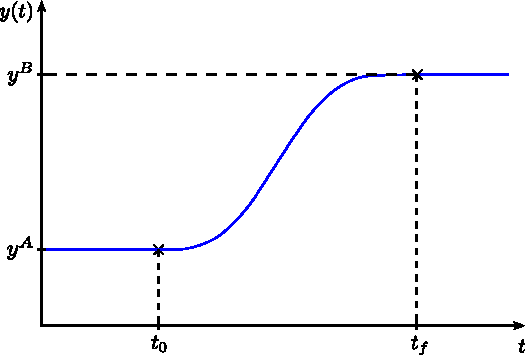
\includegraphics[scale=1]{img/state_transition.pdf}
\caption{Smooth state transition from $y^A$ to $y^B$}
\end{figure}
\subsection{Polynomials} \label{sec:polynomials}
A simple way of defining a trajectory between two points in time is a polynomial $y_d(t)=\sum_{i=0}^{2d+1}c_i\frac{t^i}{i!}$ of degree $2d+1$, where $2d+2$ is the number of boundary conditions it has to fulfill. $y_d(t)$ and its successive derivatives up to order $d$ can be written down in matrix form:
\begin{align}
\label{eq:1}
\underbrace{\begin{pmatrix}
y_d(t) \\ \dot{y}_d(t) \\ \vdots \\ y_d^{(d-1)}(t) \\ y_d^{(d)}(t)
\end{pmatrix}}_{=:\mathbf{Y}_d(t) \in \R^{(d+1)}}
=\underbrace{\begin{pmatrix}
1 &t & \frac{t^2}{2!}&         &  \hdots         &  & \frac{t^{2d+1}}{(2d+1)!} \\
0 &1   & t             &         &  \hdots         &  & \frac{t^{2d}}{(2d)!} \\
0 &0   & 1               &         & \hdots          &  &  \frac{t^{2d-1}}{(2d-1)!} \\
\vdots &                 &  \ddots & \ddots &  &   &  \vdots \\
0      &\hdots           & \hdots       & 0 & 1& \hdots & \frac{t^{d}}{(d)!} \\
\end{pmatrix}}_{=:\mathbf{T}(t)\in \R^{(d+1)\times (2d+2)}}
\underbrace{
\begin{pmatrix}
c_0 \\ c_1 \\ \vdots \\ c_{2d-1}\\ c_{2d}\\ c_{2d+1} 
\end{pmatrix}}_{=:\mathbf{c}\in \R^{(2d+2)}}
\end{align}
To calculate the parameter vector $\mathbf{c}$, the boundary conditions of the trajectory have to be defined up to degree $d$:
\begin{align*}
\underbrace{\begin{pmatrix} y_d(t_0) \\ \dot{y}_d(t_0) \\ \vdots \\ y_d^{(d)}(t_0) \end{pmatrix}}_{:=\mathbf{Y}_d(t_0)}
&\overset{!}{=}
\underbrace{\begin{pmatrix} y^A \\ \dot{y}^A \\ \vdots \\ y^{(d)A}  \end{pmatrix}}_{:=\mathbf{Y}^A}
&&&
\underbrace{\begin{pmatrix} y_d(t_f) \\ \dot{y}_d(t_f) \\ \vdots \\ y_d^{(d)}(t_f) \end{pmatrix}}_{:=\mathbf{Y}_d(t_f)}
&\overset{!}{=}
\underbrace{\begin{pmatrix} y^B \\ \dot{y}^B \\ \vdots \\ y^{(d)B}  \end{pmatrix}}_{:=\mathbf{Y}^B}
\end{align*}
This leads to a linear equation system:
\begin{align*}
\begin{bmatrix}
\mathbf{Y}_d(t_0) \\
\mathbf{Y}_d(t_f) 
\end{bmatrix}
=
\begin{bmatrix}
\mathbf{Y}^A \\
\mathbf{Y}^B
\end{bmatrix}
&=
\begin{bmatrix}
\mathbf{T}(t_0) \\
\mathbf{T}(t_f) 
\end{bmatrix}
\mathbf{c}
\end{align*}
Because $\begin{bmatrix}
\mathbf{T}(t_0) \\
\mathbf{T}(t_f) 
\end{bmatrix}$ is quadratic and not singular for $t_0,t_f\neq 0$, this linear equation system can be solved explicitly:
\begin{align}
\label{eq:2}
\mathbf{c} &= \begin{bmatrix}
\mathbf{T}(t_0) \\
\mathbf{T}(t_f) 
\end{bmatrix}^{-1}
\begin{bmatrix}
\mathbf{Y}^A \\
\mathbf{Y}^B
\end{bmatrix}
\end{align}
Because the calculation of the invertible matrix is computationally expensive, in an implementation, it is more efficient to use a linear equation system solver, like \texttt{linalg.solve()} from \emph{Numpy}, to solve for $\mathbf{c}$

$\mathbf{Y}_d(t)$ can be calculated in a closed form:
\begin{align}
\label{eq:3}
\mathbf{Y}_d(t)=\mathbf{T}(t)\mathbf{c} \quad t \in [t_0,t_f] 
\end{align}
The full trajectory can be defined as a piecewise-defined function:
\begin{align}
y_d(t)=\begin{cases}y^A & \textrm{if } t<t_0 \\ \sum_{i=0}^{2d+1}c_i\frac{t^i}{i!} & \textrm{if } t\in [t_0,t_f] \\y^B & \textrm{if } t>t_f\end{cases}
\end{align}
\subsection{Polynomials using a prototype function}
A slightly different approach for a polynomial reference trajectory $y_d(t)$ is again a piecewise-defined function:
\begin{align}
\label{eq:5}
y_d(t) = \begin{cases} y^A &\textrm{if } t<t_0 \\ y^A + (y^B-y^A)\varphi_\gamma\left(\frac{t-t_0}{t_f-t_0}\right) &\textrm{if } t \in [t_0, t_f] \\y^B &\textrm{if } t>T\end{cases}
\end{align}
$\tau \rightarrow \varphi_\gamma(\tau)$ is a protoype function, where $\gamma$ indicates how often $\varphi_\gamma(\tau)$ is continuously differentiable. The function has to meet the following conditions, such that the reference trajectory is feasible:
\begin{subequations}
\label{eq:6}
\begin{align}
\varphi_\gamma(0)=0 \quad \varphi^{(j)}_\gamma(0)=0 \quad j = 1,...,\gamma \\
\varphi_\gamma(1)=1 \quad \varphi^{(j)}_\gamma(1)=0 \quad j = 1,...,\gamma 
\end{align}
\end{subequations}
An approach for the derivative of $\varphi_\gamma(\tau)$, which meets the conditions \eqref{eq:6} is:
\begin{align}
\frac{\d \varphi_\gamma(\tau)}{\d \tau} = \alpha \frac{\tau^{\gamma}}{\gamma!}\frac{(1-\tau)^{\gamma}}{\gamma!}
\end{align}
Integration leads to:
\begin{align}
\varphi_\gamma(\tau) = \alpha \int_0^\tau\frac{\tilde{\tau}^{\gamma}}{\gamma!}\frac{(1-\tilde{\tau})^{\gamma}}{\gamma!} \d \tilde{\tau}
\end{align}
After $\gamma$ partial integrations we get:
\begin{align*}
\varphi_\gamma(\tau)= \frac{\alpha}{(\gamma!)^2} \sum_{k=0}^{\gamma} \binom{\gamma}{k} \frac{(-1)^k\tau^{\gamma+k+1}}{(\gamma+k+1)}
\end{align*}
To solve for the unknown $\alpha$, the  condition $\varphi_\gamma(1)\overset{!}{=}1$ is used:
\begin{align*}
\varphi_\gamma(1)= &\frac{\alpha}{(\gamma!)^2} \sum_{k=0}^{\gamma} \binom{\gamma}{k} \frac{(-1)^k}{(\gamma+k+1)} \overset{!}{=} 1 \\
\Leftrightarrow \quad & \alpha = (2\gamma+1)!
\end{align*}
Finally the prototype function is defined as:
\begin{align}
\varphi_\gamma(\tau)= \frac{(2\gamma+1)!}{(\gamma!)^2} \sum_{k=0}^{\gamma} \binom{\gamma}{k} \frac{(-1)^k\tau^{\gamma+k+1}}{(\gamma+k+1)}
\end{align}
and it's $n$-th derivative:
\begin{align}
\varphi_\gamma^{(n)}(\tau)= \frac{(2\gamma+1)!}{(\gamma!)^2} \sum_{k=0}^{\gamma} \left(\binom{\gamma}{k} \frac{(-1)^k\tau^{\gamma+k-n+1}}{(\gamma+k+1)}\prod_{i=1}^n(\gamma+k-i+2)\right)
\end{align}
In the last step the $n$-th derivative of \eqref{eq:5} $(n=1,...,\gamma$) is derived.
\begin{align}
y_d^{(n)}(t) = \begin{cases} y_d^{(n)}(t_0) & \textrm{if } t<t_0 \\ 
y_d^{(n)} + \sum_{i=0}^{n}\binom{n}{i}(y_d^{(n-i)}(t)-y_d^{(n-i)}(t_0))\left(\frac{1}{t_f-t_0}\right)^i\varphi_\gamma^{(i)}\left(\frac{t-t_0}{t_f-t_0}\right) &\textrm{if } t \in [t_0, t_f] \\ 
y_d^{(n)}(t_f)&\textrm{if } t>t_f\end{cases}
\end{align}
The main difference of this method over the one presented in \ref{sec:polynomials} is, that no linear equation system has to be solved. This can have runtime advantages when applied on a real system.
\subsection{Gevrey-functions}
It is sometimes necessary, that a planned trajectory is infinitely differentiable \footnote{For example when you are controling an infinite dimensional system.}. A polynomial approach can't be used in this case, because an infinite number of parameters is needed to construct such a polynomial. One approach to deal with this problem is to use so called Gevrey-funtions.
\begin{defi}[Gevrey-function] A function $y(t):\Omega \mapsto \R$ is called a Gevrey-function of order $\alpha$, if $y(t) \in C^\infty(\Omega)$ and positive constants $M, R$ exist, such that
\begin{align*}
\sup_{t\in\Omega}{|y^{(n)}(t)| \leq \frac{M}{R^n}(n!)^\alpha}.
\end{align*}
\end{defi}
One function that belongs to the Gevrey class of functions is:
\begin{align}
\tan(blala)
\end{align}
\subsection{Implementation in \py}
In order to automate the process of trajectory planning at first a \emph{Planner} base class is implemented. Then a new subclass for each new planning algorithm is created.

\textbf{\py source code file: \texttt{Planner.py}}
\subsubsection{The \emph{Planner} base class}
A \emph{Planner} should have the following attributes:
\begin{itemize}
	\item[] \texttt{YA} - vector of $y$ and it's derivatives up to order \texttt{d} at start time \texttt{t0}
	\item[] \texttt{YB} - vector of $y$ and it's derivatives up to order \texttt{d} at final time \texttt{tf}
	\item[] \texttt{t0} - start time of the point-to-point transition
	\item[] \texttt{tf} - final time of the point-to-point transition
	\item[] \texttt{d} - planned trajectory should be smooth up to the $d$-th derivative
\end{itemize}
The planned trajectory has to be evaluated at runtime, but how the this functionality should be implemented, should be defined in the specific subclass. By using in abstract base class method, we force a subclass of \emph{Planner} to have a method \texttt{eval()}.
\listcodeplanner{2}{27}
\subsubsection{The \emph{PolynomialPlanner} subclass}
\label{sec:polynomialplanner}
To implement the planning algorithm that was developed in \autoref{sec:polynomials}, a new class \texttt{PolynomialPlanner} is created that inherits from the previously defined class \texttt{Planner}. All the attributes and methods of \texttt{Planner} are now also attributes and methods of \texttt{PolynomialPlanner}.
\listcodeplanner{28}{33}
To solve for the parameter vector $\mathbf{c}$, the matrix $\mathbf{T}(t)$ from \eqref{eq:1} is calculated and a method \texttt{TMatrix()} is therefore created:
\listcodeplanner{73}{94}
Then a method, that solves \eqref{eq:2} and returns the parameter vector $\mathbf{c}$ is needed:
\listcodeplanner{97}{116}
Because the parameters don't change, ones they are calculated, a new attribute \texttt{c} is created:
\listcodeplanner{35}{79}
Finally a method \texttt{eval()} that implements \eqref{eq:3} is defined:
\listcodeplanner{39}{54}
as well as a second method \texttt{eval\_vec()}, that can handle a time array as an input:
\listcodeplanner{57}{70}
The polynomial trajectory planner is now successfully implemented and can be tested.

\textbf{Example:}

\textbf{\py source code file: \texttt{01\_trajectory\_planning.py}}

Suppose a trajectory from $y(t_0)=0$ to $y(t_f) = 1$ with $t_0=1s$ and $t_f = 2s$ has to be planned. The trajectory should be smoothly differentiable twice $(d=2)$. Therefore the boundary conditions for the first and second derivative of $y$ have to be defined: 
\begin{align*}
\dot{y}(t_0)=0 &&& \dot{y}(t_f)=0 \\
\ddot{y}(t_0)=0 &&& \ddot{y}(t_f)=0 \\
\end{align*}
The total time interval for the evaluation of the trajectory is $t\in[0s,3s]$.

At first the boundary conditions for $t=t_0$ and $t=t_f$ are set:
\listcodeplanning{7}{8}
After that the start and final time of the transition and the total time interval:
\listcodeplanning{9}{11}
Then $d$ is set and a \texttt{PolynomialPlanner} instance \texttt{yd} with the defined parameters is created.
\listcodeplanning{12}{13}
The calculated parameters can be displayed
\listcodeplanning{15}{16}
and the generated trajectory at the defined total time interval can be sampled
\listcodeplanning{18}{19}
At last, the results are plotted.
\listcodeplanning{21}{27}
\begin{figure}[ht]
\centering
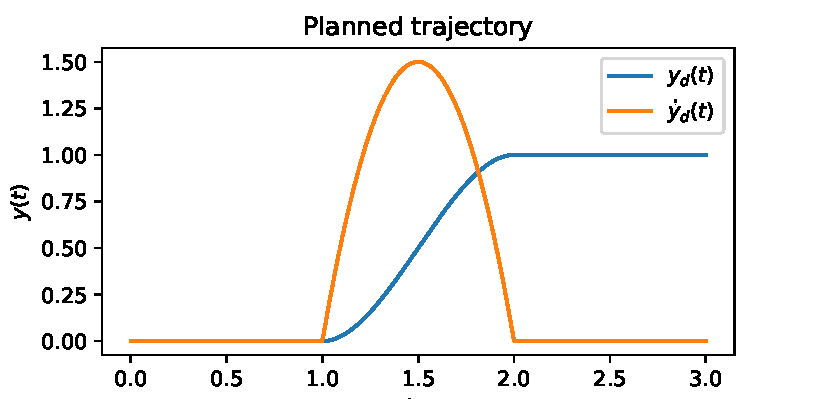
\includegraphics[scale=0.9]{img/planned_trajectory.pdf}
\end{figure}
\subsubsection{The \emph{PrototypePlanner} subclass}
Implementation can be found in the file.
\newpage
\section{Feedforward control design}
\label{sec:ffcontrol}
\textbf{\py source code file: \texttt{02\_car\_feedforward\_control.py}}

Recapture the model of the car from tutorial 1 \footnote{\url{https://github.com/TUD-RST/pytutorials/tree/master/01-System-Simulation-ODE}}, parameterized in time $t$:
\begin{subequations}
\begin{align}
\dot y_1 &= v \cos(\theta)\\
\dot y_2 &= v \sin(\theta)\\
\dot \theta &= \frac{v}{l}\tan(\varphi).
\end{align}
\end{subequations}
\subsection{Reparameterization of the model}
The model of the car has to be parameterized in arc length $s$ to take care of singularities, that would appear in steady-state $(v=0)$.

The following can be assumed:
\begin{align*}
\frac{\d}{\d t} = \frac{\d}{\d t}\frac{\d s}{\d s} = \frac{\d}{\d s}\frac{\d s}{\d t} = \frac{\d}{\d s}\dot s
\end{align*}
Replacing $\frac{\d}{\d t}$ in the model equations leads to:
\begin{subequations}
\begin{align}
\frac{\d}{\d s}\dot s y_1 &= v \cos(\theta)\\
\frac{\d}{\d s}\dot s y_2 &= v \sin(\theta)\\
\frac{\d}{\d s}\dot s \theta &= \frac{v}{l}\tan(\varphi).
\end{align}
\end{subequations}
\begin{align}
v = |\dot{\bm{y}}| = \sqrt{\dot y_1^2+\dot y_2^2}
\end{align}
This equation is parameterized in $s$:\footnote{assuming $\dot s > 0$} 
\begin{align}
v = \sqrt{(\frac{\d}{\d s}\dot sy_1)^2+(\frac{\d}{\d s}\dot s y_2)^2}=\dot s \sqrt{(y_1^\prime)^2+(y_2^\prime)^2}
\end{align}
 
If $s$ is the arc length, the Pythagorean theorem $ds^2 = dy_1^2 + dy_2^2$ leads to:
\begin{subequations}
\begin{align}
&1 = \left(\frac{dy_1}{ds}\right)^2 + \left(\frac{dy_2}{ds}\right)^2  \\
\Leftrightarrow \quad & 1 = \sqrt{(y_1^\prime)^2+(y_2^\prime)^2}
\end{align}
\end{subequations}
Therfore $v=\dot s$. 
The system paramterized in $s$ is given by:
\begin{subequations}
\begin{align}
y_1^\prime &= \cos(\theta)\\
y_2^\prime &= \sin(\theta)\\
\theta^\prime &= \frac{1}{l}\tan(\varphi).
\end{align}
\end{subequations}
\subsection{Deriving feedforward control laws}
Goal: Drive the car in the $y_1$-$y_2$-plane frome a point $(\yIZ, \yIIZ)$ to a point $(\yIT, \yIIT)$ in time $T=t_f-t_0$. The car should be in rest at the beginning and at the end of the process and the trajectory is defined by a sufficiently smooth function $f : \mathbb{R} \to \mathbb{R}$ with $y_2 = f(y_1)$. Note that $(y_1, y_2)$ is a flat output of the system.

\textbf{Step 1:} Calculate the dependency of the remaining system variables $\theta$ and $\varphi$ of the  length parameterized system on $(y_1, y_2)$:
\begin{align}
\tan(\theta) &= \frac{y_2^\prime}{y_1^\prime} = \diff{y_2}{y_1} = f^\prime(y_1)\\
(1 + \tan^2(\theta))\diff{\theta}{y_1} &= f^{\prime\prime}(y_1) \nonumber \\
\Leftrightarrow \quad \diff{\theta}{y_1}&= \frac{f^{\prime\prime}(y_1)}{1 + (f^\prime(y_1))^2} = \frac{\theta^\prime}{y_1^\prime} \nonumber\\
\intertext{with $(y_1^\prime)^2 + (y_2^\prime)^2 = 1 \, \Leftrightarrow \, y_1^\prime = 1/\sqrt{1 + (f^\prime(y_1))^2}$ one obtains:}
\Leftrightarrow \quad \theta^\prime &= \frac{f^{\prime\prime}(y_1)}{\left(1 + (f^\prime(y_1))^2\right)^{3/2}}\\
\tan(\varphi) &= l\theta^\prime = \frac{lf^{\prime\prime}(y_1)}{\left(1 + (f^\prime(y_1))^2\right)^{3/2}}
\end{align}

Result: Depending on the planning $y_2 = f(y_1)$ the required steering angle can be calculated solely from $y_1$ and derivatives of $f$ w.r.t.~$y_1$ up to order 2. The planned trajectory has to fulfill the following boundary conditions:
\begin{align*}
f(\yIZ) = \yIIZ &&& f(\yIT) = \yIIT \\
f^\prime(\yIZ) = \tan(\theta_A) &&& f^\prime(\yIT) = \tan(\theta_B) \\
f^{\prime\prime}(\yIZ) = (1+\tan^2(\theta_A))\left(\frac{\frac{1}{l}\tan(\varphi_A)}{cos(\theta_A)}\right) &&& 
f^{\prime\prime}(\yIT) = (1+\tan^2(\theta_B))\left(\frac{\frac{1}{l}\tan(\varphi_B)}{cos(\theta_B)}\right) 
\end{align*}
By always setting $\varphi_A=\varphi_B=0$, these conditions simplify to:
\begin{align*}
f^{\prime\prime}(\yIZ) = 0 &&& f^{\prime\prime}(\yIT) = 0
\end{align*}
\textbf{Step 2:} Calculation of the required velocity $v$. Another function $g: \mathbb{R} \to \mathbb{R}$ is defined, with $y_1 = g(t)$ and $g(t_0) = \yIZ$, $\dot g(t_0) = 0$, $g(t_f) = \yIT$, $\dot g(t_f) = 0$. 
\begin{align}
v &= \sqrt{\dot y_1^2 + \dot y_2^2} = \dot y_1\sqrt{1 + (f^\prime(y_1))^2} = \dot g(t) \sqrt{1 + (f^\prime(g(t)))^2}
\end{align}

Hence, the overall, time parameterized feedforward control reads:
\begin{subequations}
\label{eq:controllaw}
\begin{align}
v(t) &= \dot g(t) \sqrt{1 + (f^\prime(g(t)))^2}\\
\varphi(t) &= \arctan\left(\frac{lf^{\prime\prime}(g(t))}{\left(1 + (f^\prime(g(t)))^2\right)^{3/2}}\right)
\end{align}
\end{subequations}
Or expressed in $s$:
\begin{subequations}
\label{eq:controllaw_2}
\begin{align}
v(s) &= \dot{s} \sqrt{y_2^{\prime2}+y_1^{\prime2}}\\
\varphi(s) &= \arctan\left(l \frac{y_2^{\prime\prime}y_1^\prime-y_1^{\prime\prime}y_2^\prime}{(y_1^{\prime2}+y_2^{\prime2})^{\frac{3}{2}}}\right) = \arctan\left(l (y_2^{\prime\prime}y_1^\prime-y_1^{\prime\prime}y_2^\prime)\right)
\end{align}
\end{subequations}
If polynomials are chosen for the two functions $f$ and $g$ it has to be ensured that $f$ is of order 3 and $g$ of order 2 to make sure the control law is smooth. The resulting $f(g)$ is of order 5.
\subsection{Implementation}
For the implementation of the controller, a the polynomial planner from \ref{sec:polynomialplanner} is used.
At first all necessary simulation parameters are defined:
\listcodeffcontrol{21}{27}
Initialization of the trajectory planners:
\listcodeffcontrol{30}{45}
Implementation of the the control law:
\listcodeffcontrol{70}{95}
Running the simulation:
\listcodeffcontrol{298}{298}
The results can be extracted by:
\listcodeffcontrol{299}{299}
To get the control vector can be done by evaluating \texttt{control()} with the simulated trajectory and recalculate the values that were applied to the system. 
\listcodeffcontrol{300}{302}
Because \texttt{control()} works only for scalar time values, this has to be done in a \texttt{for}-loop.
Plotting the simulation results and the reference trajectories:
\listcodeffcontrol{307}{318}
\texttt{plot\_data()} was adopted to also plot \texttt{x\_ref}. The changes can be found in the corrosponding file.
\subsubsection{Result}
\label{subsec:result}
As an example, the transition from $(0, 0, 0)$ to $(5, 5, 0)$, starting at $t=1s$ ending at $t=9s$ is shown in \autoref{fig:control_trajectory}. The whole simulation time interval goes from $t=0s$ to $t=10s$.
The animation shows the behaviour of the car in the plane:
\begin{figure}[ht]
\centering
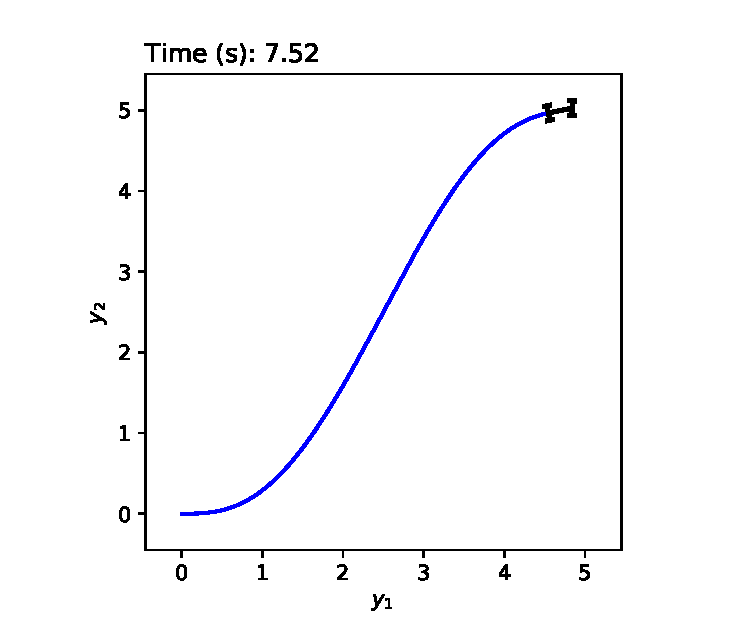
\includegraphics[scale=1]{img/plane_trajectory.pdf}
\caption{Smooth state transition from $y^A$ to $y^B$ in the plane}
\label{fig:plane_trajectory}
\end{figure}
\begin{figure}[ht]
\centering
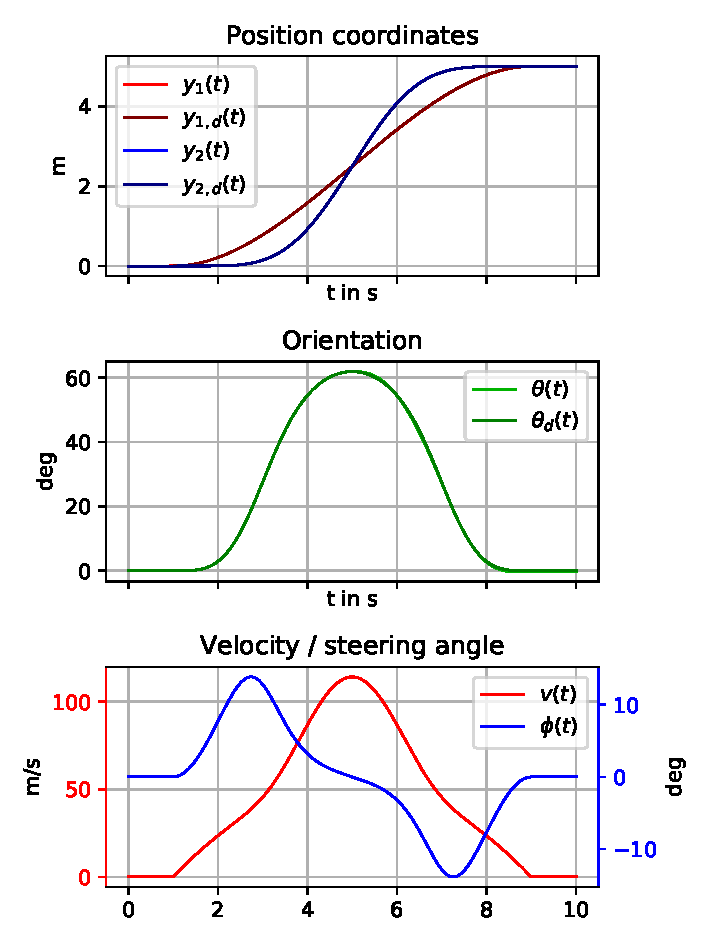
\includegraphics[scale=1]{img/control_trajectory.pdf}
\caption{Feedforward control without model errors}
\label{fig:control_trajectory}
\end{figure}
\clearpage
\section{Feedback control design}
\label{sec:fbcontrol}
\textbf{\py source code file: \texttt{03\_car\_feedback\_control.py}}

In \autoref{sec:ffcontrol} the controller acts on the exact same system as it was designed for, but in the real world, model errors are inevidable and a feedforward control is not sufficient. Assuming the length of the car in the controller $\tilde{l}$ differs from the real car length $l$ by a factor of $0.9$, the feedfoward control of \ref{subsec:result} shows a bad performance, as can be seen in \autoref{fig:failed_control}. 
\subsection{Deriving feedback control laws}
To account for model errors, a feedback controller has to be designed to fulfill the objective. This is done by a feedback linearization.
The linearization is done by introducing new inputs $w_1$ and $w_2$:
\begin{align}
\label{eq:new_inputs}
w_1 = y_1^\prime \qquad w_2 = y_2^{\prime\prime}
\end{align}
This leads the linear system shown in \autoref{fig:linear_system}. 
\begin{figure}[ht]
\centering
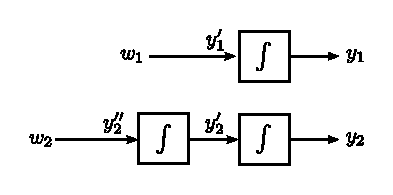
\includegraphics[scale=1]{img/linear_system.pdf}
\caption{Block diagram of the linearized system}
\label{fig:linear_system}
\end{figure}
The tracking error $e$ is defined as:
\begin{align}
\label{eq:error}
e_i = y_i-y_{i,d} \qquad i = 1,2
\end{align}
A differential equation for the error term can be defined:
\begin{align}
\label{eq:error_ode}
0 = e_i^{\prime\prime}+k_{1i}e_i^{\prime}+k_{0i}e_i \qquad i = 1,2 \quad k_{0i},k_{1i} \in \R^+
\end{align}
Substituting \eqref{eq:new_inputs} and \eqref{eq:error} in \eqref{eq:error_ode} leads to:
\begin{subequations}
\begin{align}
w_1 =  y_{1,d}^\prime - k_{01}(y_{1}-y_{1,d}) \\
w_2 = y_{2,d}^{\prime\prime}  - k_{02}(y_{2}^\prime-y_{2,d}^\prime) - k_{02}(y_{2}-y_{2,d})
\end{align}
\end{subequations}
\begin{figure}[ht]
\centering
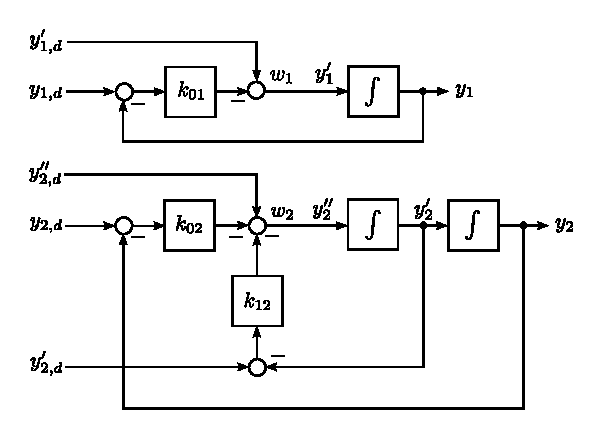
\includegraphics[scale=1]{img/linear_system_feedback.pdf}
\caption{Block diagram of the feedback system}
\label{fig:linear_system_feedback}
\end{figure}
These equations are substituted into \eqref{eq:controllaw_2} to obtain the feedback control law:
\begin{subequations}
\begin{align}
v(s) &= \dot{s}_d\\
\varphi(s) &= \arctan\left(l (w_2w_1-y_1^{\prime\prime}y_2^\prime)\right)
\end{align}
\end{subequations}
where $\dot{s}_d$ is the desired velocity  and $y_1^{\prime\prime} = 0$.
To reparametrize these control laws in time, the desired trajectories are expressed in $f$ and $g$:
\begin{subequations}
\begin{align*}
y_{1,d} &= g(t)  &&& y_{2,d} &= f(g(t))\\
y_{1,d}^\prime &= \frac{1}{\sqrt{1+(f^{\prime }(g(t)))^2}} &&& y_{2,d}^\prime &= \frac{f^{\prime }(g(t))}{\sqrt{1+(f^{\prime }(g(t)))^2}}\\
\dot{s}_d &= v_d(t) = \dot g(t) \sqrt{1 + (f^\prime(g(t)))^2}&&& y_{2,d}^{\prime\prime} &= \frac{f^{\prime \prime}(g(t))}{1+(f^{\prime }(g(t)))^2}
\end{align*}
\end{subequations}
\subsection{Implementation}
To implement the controller, at first the controller parameters are defined:
\listcodefbcontrol{91}{94}
The controller parameters have to be hand tuned and must be $>0$ for the system to be stable.

Then the desired trajectories are expressed in the planner trajectories $f$ and $g$:
\listcodefbcontrol{103}{109}
Afterwards $w_1$ and $w_2$ are set:
\listcodefbcontrol{111}{113}
In the final step, the control laws are calculated and return from the function:
\listcodefbcontrol{115}{120}
\subsubsection{Result}
The experiment from \ref{subsec:result} is repeated with the same model error as in \autoref{fig:failed_control}, but now using the feedback controller instead. As it can be seen in \autoref{fig:success_control} the control objective of following the planned trajectory succeeded, even with model errors.
\begin{figure}[ht]
\centering
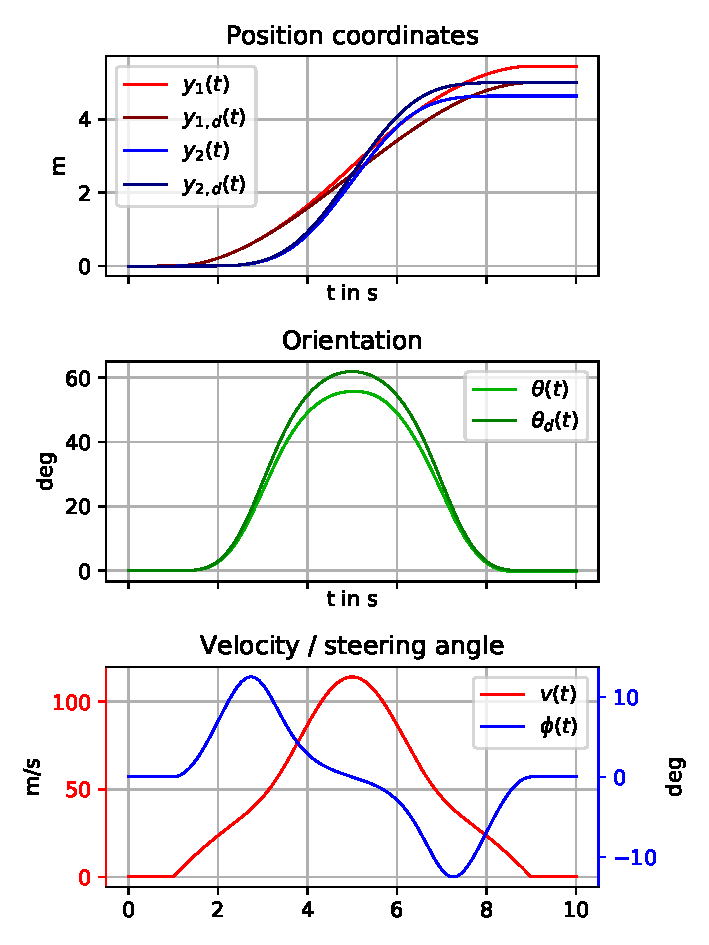
\includegraphics[scale=1]{img/failedcontrol.pdf}
\caption{Feedfoward control for $\tilde{l}=0.9l$}
\label{fig:failed_control}
\end{figure}
\begin{figure}[ht]
\centering
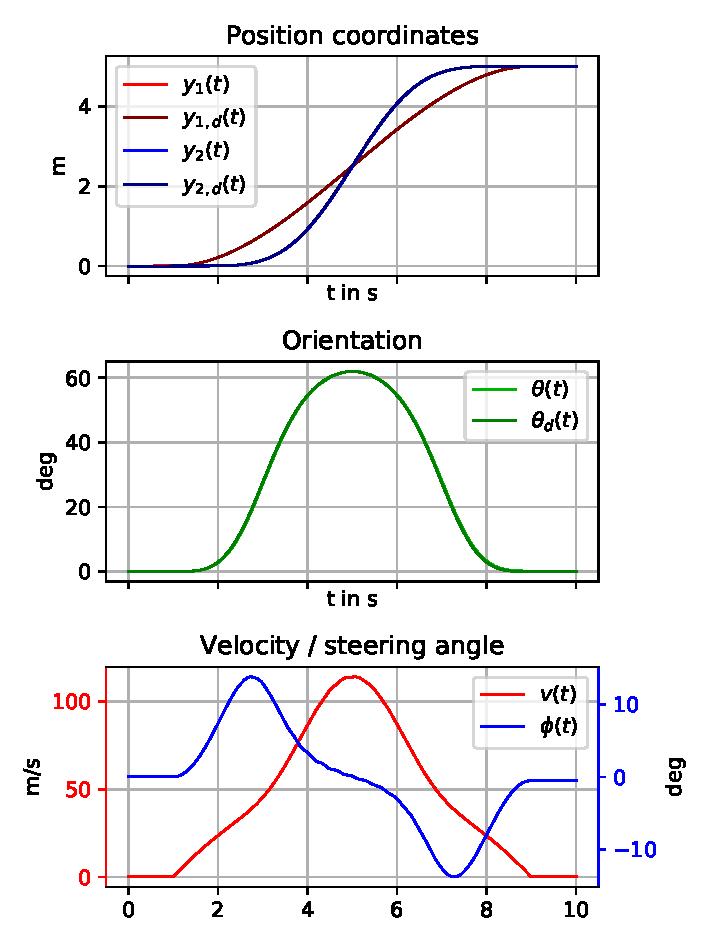
\includegraphics[scale=1]{img/successcontrol.pdf}
\caption{Feedback control for $\tilde{l}=0.9l$}
\label{fig:success_control}
\end{figure}
\printglossaries
\end{document}

%%% Local Variables:
%%% mode: latex
%%% TeX-master: t
%%% End:
